\onecolumn
\thispagestyle{empty}
\hbox{}
\vspace{160pt}

\noindent
\makebox[0pt][l]{\rule[0pt]{70pt}{70pt}}%
\rule{\textwidth}{8pt}
\\[-56pt]
\noindent
\hbox{}
\hspace{76pt}
{\LARGE \textsc{tma}\textit{4110}}
\\[5pt]
\hbox{}
\hspace{76pt}
{\HUGE\textbf{Matematikk 3}}
\\[18pt]
\hbox{}
\hfill
{\large Notater høsten 2018}\hspace{2pt}

\vspace{80pt}

\begin{center}
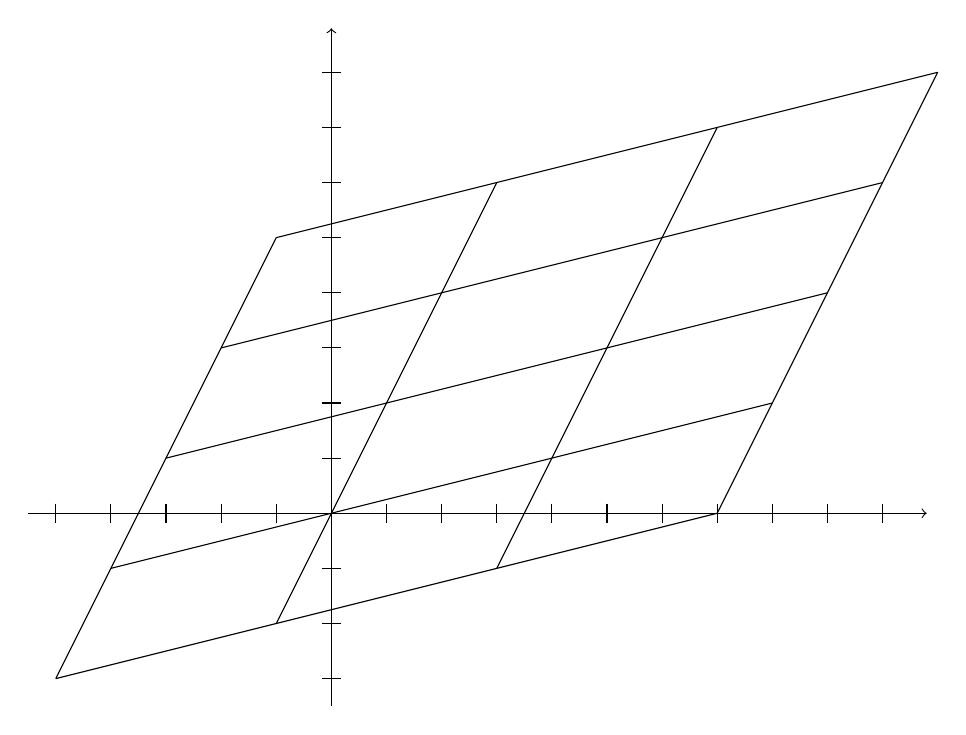
\begin{tikzpicture}[scale=.7]
\draw[->] (-5.5,0) -- (10.8,0);
\draw[->] (0,-3.5) -- (0,8.8);
\foreach \x in {-5,-4,-3,-2,-1,1,2,3,4,5,6,7,8,9,10}
\draw (\x,5pt) -- (\x,-5pt);
\foreach \y in {-3,-2,-1,1,2,3,4,5,6,7,8}
\draw (5pt,\y) -- (-5pt,\y);
\draw (-5,-3) -- (7,0);
\draw (-4,-1) -- (8,2);
\draw (-3,1) -- (9,4);
\draw (-2,3) -- (10,6);
\draw (-1,5) -- (11,8);
\draw (-5,-3) -- (-1,5);
\draw (-1,-2) -- (3,6);
\draw (3,-1) -- (7,7);
\draw (7,0) -- (11,8);
% \filldraw (4,1) circle [radius=4pt] node[anchor=south east] {$b_1$};
% \filldraw (1,2) circle [radius=4pt] node[anchor=north west] {$b_2$};
% \filldraw (11,8) circle [radius=4pt] node[anchor=west] {$v$};
\end{tikzpicture}
\end{center}

\vfill
\begin{center}
\huge
\textsc{Øystein Skartsæterhagen}
\\[6pt]
\textsc{Morten Andreas Nome}
\\[6pt]
\textsc{Paul Trygsland}
\end{center}

\vspace{10pt}

\begin{center}
Disse notatene kan fritt kopieres og endres,
under betingelsene i lisensen
\href{http://creativecommons.org/licenses/by-sa/4.0/}{CC BY-SA}.
\end{center}

\vspace{2pt}

\twocolumn
